
\documentclass[12pt]{article}
\usepackage[utf8]{inputenc}
\usepackage[T1]{fontenc}
\usepackage[spanish]{babel}
\usepackage{graphicx}
\usepackage{float}
\usepackage{booktabs}
\usepackage[margin=1in]{geometry}
\usepackage{array}
\setlength{\parskip}{0.6em}
\setlength{\parindent}{0pt}


\begin{document}

\begin{titlepage}
    \centering

    \vspace*{1.5cm}

    \vspace{1.3cm}

    {\Large Tecnológico de Monterrey\par}
    \vspace{0.6cm}

    {\Huge \textbf{Proyecto Final Integrador}\par}
    \vspace{0.4cm}

    {\Large Dominio: Neuroingeniería\par}

    \vspace{2cm}

    {\large
    José Emiliano Calderón Gurubel\par
    Dana Paola Rosete Gómez\par
    José Ricardo Cañedo Verdugo\par
    Daisy Karina Núñez Flores\par
    }

    \vspace{1.5cm}

    {\large \textit{Applied Computing}\par}

    \vfill

    {\large 10 de abril de 2026\par}

\end{titlepage}

\section{Resumen}
\addcontentsline{toc}{section}{Resumen}

\vspace{0.3cm}

Este reporte presenta un análisis integrado que combina exploración de datos, pruebas estadísticas, modelos de aprendizaje automático y optimización, aplicado a características de sincronía EEG obtenidas en condiciones de lectura compartida e individual. El objetivo es evaluar si estas características, derivadas de díadas familiares, permiten discriminar entre distintos estados cognitivos asociados a cada condición. Los resultados indican que la sincronía cerebral constituye un indicador informativo para diferenciar entre lectura individual y compartida, destacando el potencial de estas métricas en el análisis de interacción cognitiva.

\vspace{0.8cm}

\section{Metodología}

El pipeline desarrollado se estructuró en módulos secuenciales que permiten transformar señales EEG crudas en resultados interpretables mediante análisis estadístico, aprendizaje automático y visualización.

En primer lugar (C1), se realizó la carga, limpieza y preprocesamiento de las señales EEG obtenidas en distintas condiciones experimentales: línea base, lectura compartida y lectura individual. A partir de estas señales, se extrajeron características de sincronía cerebral entre pares de electrodos utilizando métricas como PLI y wPLI en distintas bandas de frecuencia. Estas características se organizaron en matrices de datos para su posterior análisis.

Posteriormente, se llevó a cabo un análisis exploratorio de datos (EDA), en el cual se evaluaron diferencias entre condiciones mediante pruebas estadísticas no paramétricas. En particular, se utilizaron comparaciones entre grupos (Paired) acompañadas de corrección por múltiples pruebas (FDP), así como el cálculo del tamaño de efecto mediante la medición Cliff’s d y Wilcoxon. 

En la etapa de aprendizaje automático (C4), se entrenaron distintos modelos de clasificación, incluyendo Random Forest, Support Vector Machine (SVM) y Gradient Boosting, con el objetivo de distinguir entre condiciones experimentales a partir de las características EEG. El desempeño de los modelos se evaluó mediante métricas como exactitud, precisión y F1-score.

Adicionalmente, se consideró una etapa de optimización (C3), en la cual se exploran estrategias para mejorar el desempeño de los modelos y la selección de características, contribuyendo a una mejor generalización del sistema.

Finalmente, en el módulo de visualización e integración (C6), se generaron figuras y reportes que permiten interpretar los resultados obtenidos, incluyendo análisis de características significativas, comparaciones entre condiciones, matrices de correlación y desempeño de modelos.

En este proyecto, la comparación final se realizó entre los modelos de aprendizaje automático implementados en C4. Los módulos C2 y C5 no fueron incluidos en la tabla comparativa final debido a que, de acuerdo con la naturaleza del problema y las reglas de composición del framework para equipos de este tamaño, C2 no resultó aplicable y C5 fue omitido justificadamente.

\section{Resultados del análisis exploratorio (C1)}
\begin{figure}[H]
    \centering
    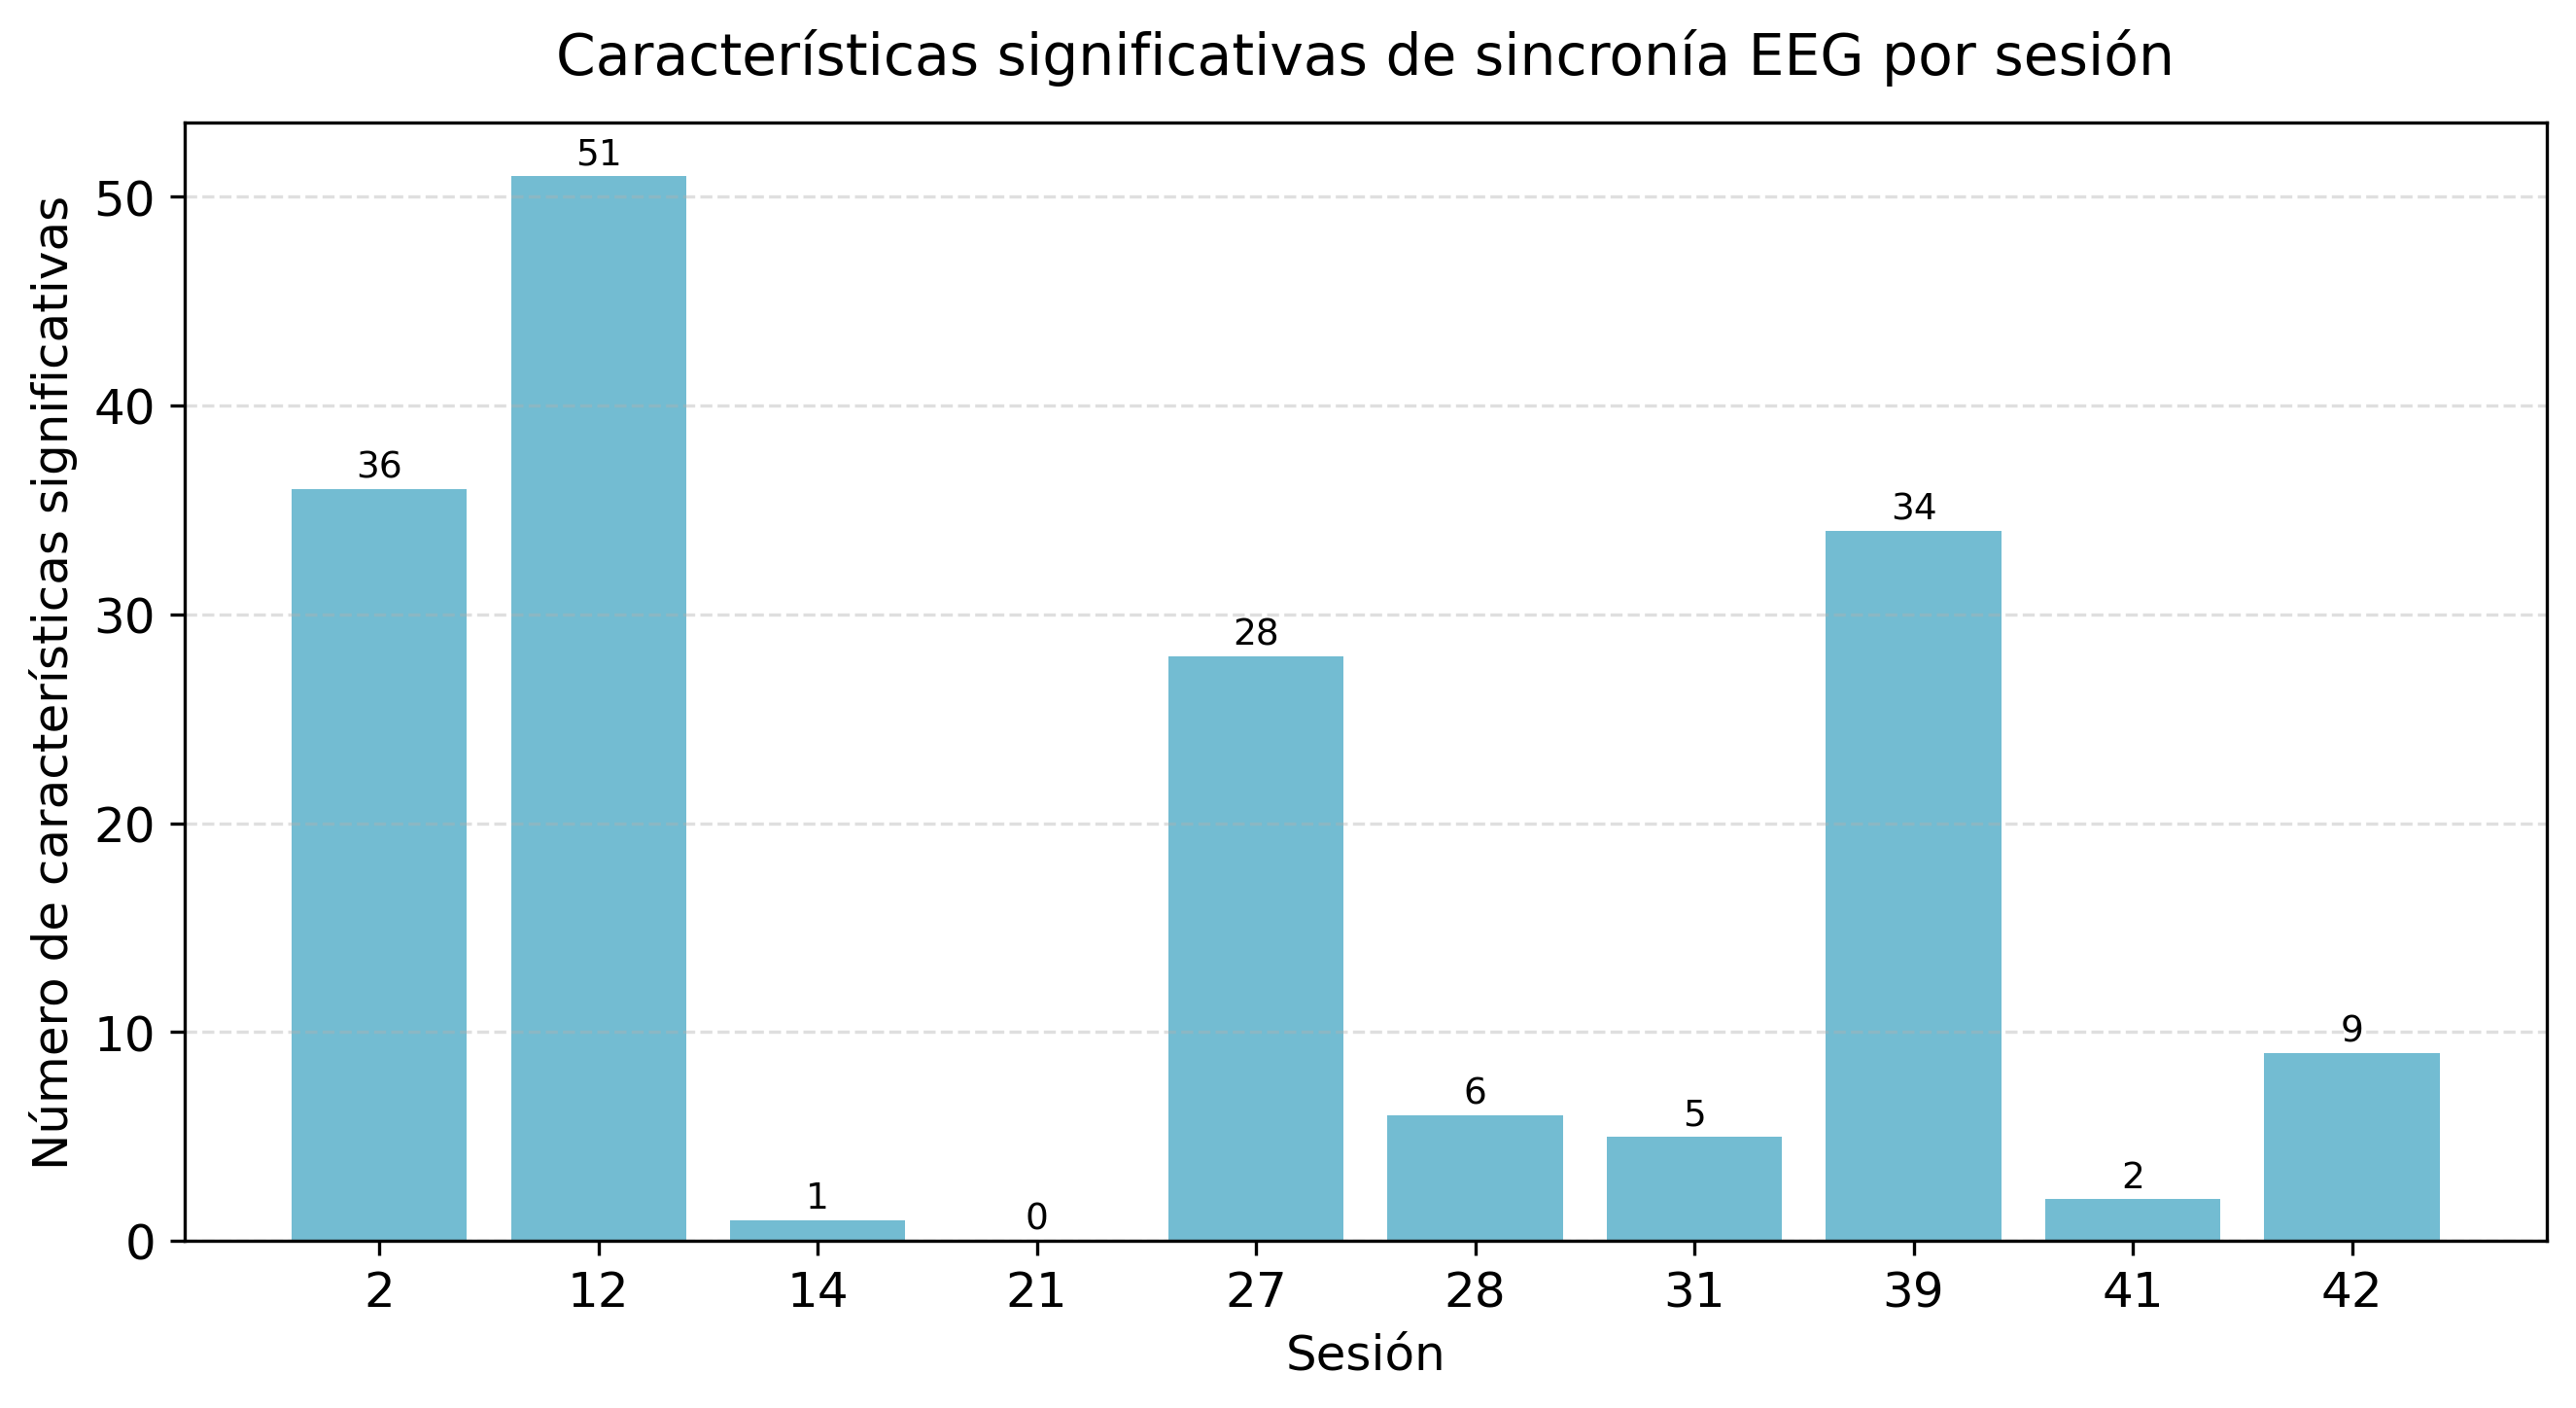
\includegraphics[width=0.8\textwidth]{figures/eda/significant_features_by_session.png}
    \caption{Número de características de sincronía EEG estadísticamente significativas por sesión.}
\end{figure}

\begin{figure}[H]
    \centering
    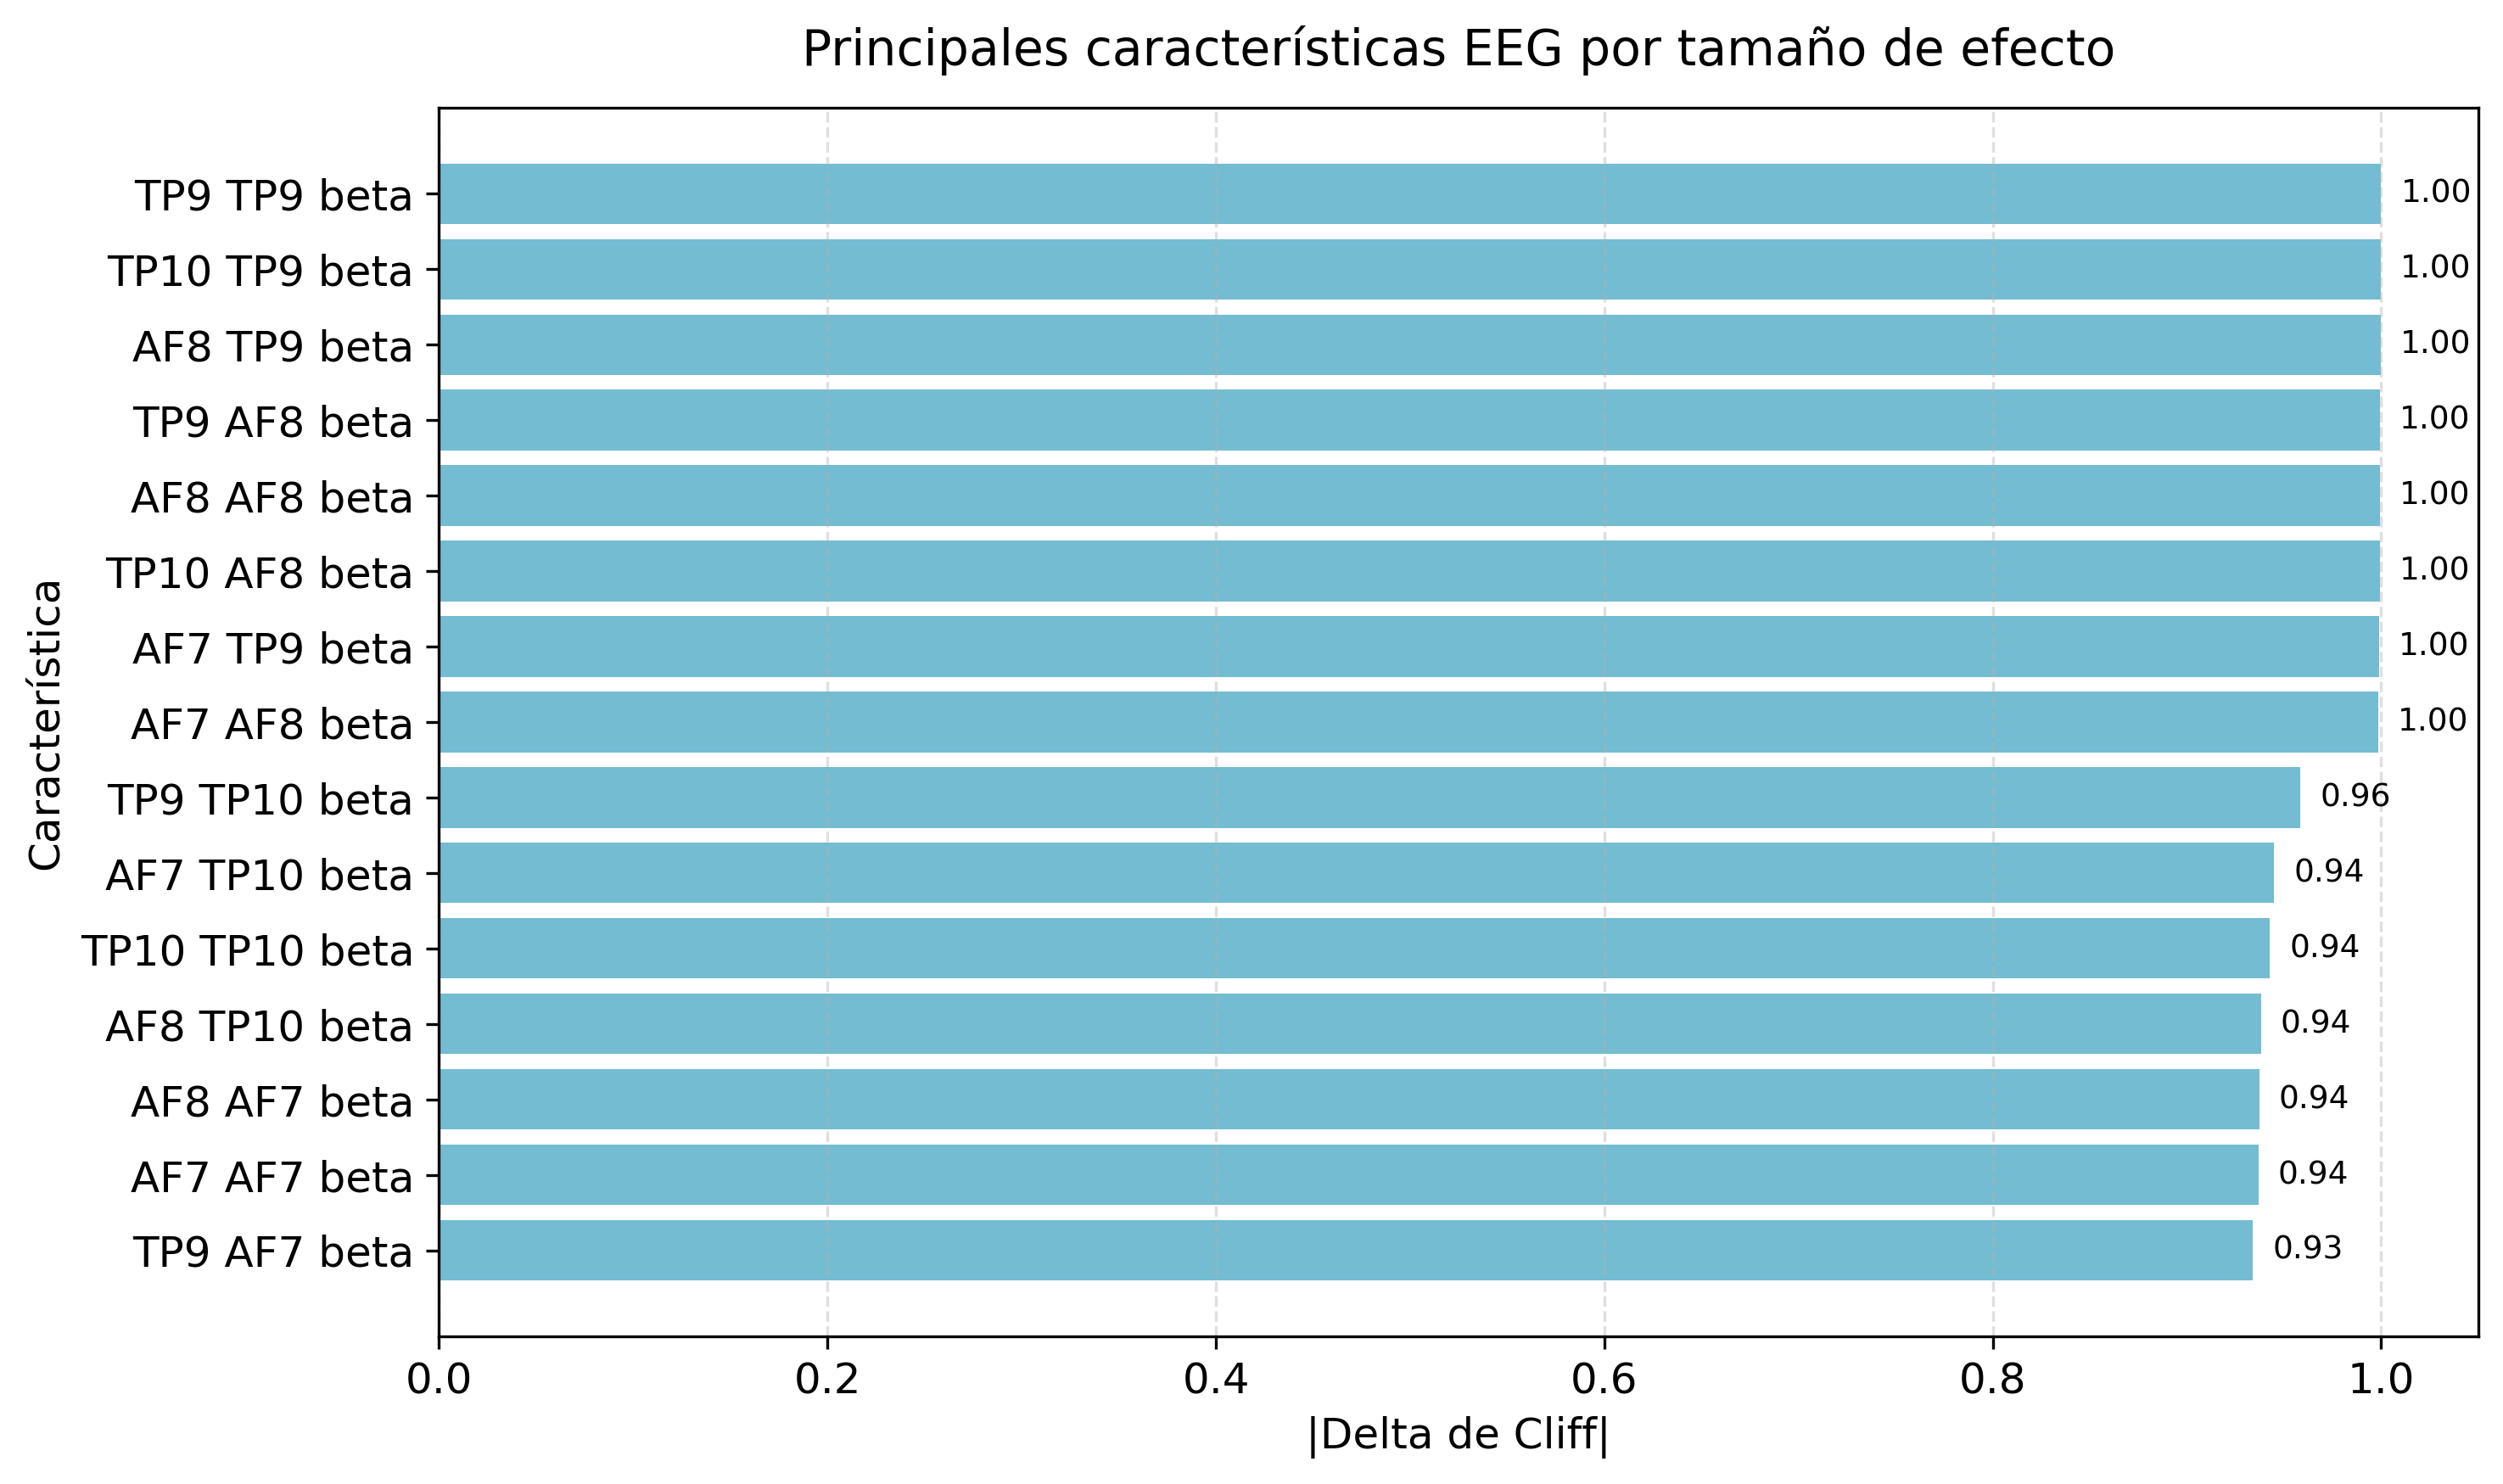
\includegraphics[width=0.9\textwidth]{figures/eda/top_effect_sizes.png}
    \caption{Principales características EEG ordenadas por magnitud del tamaño de efecto absoluto (Delta de Cliff).}
\end{figure}

\begin{figure}[H]
    \centering
    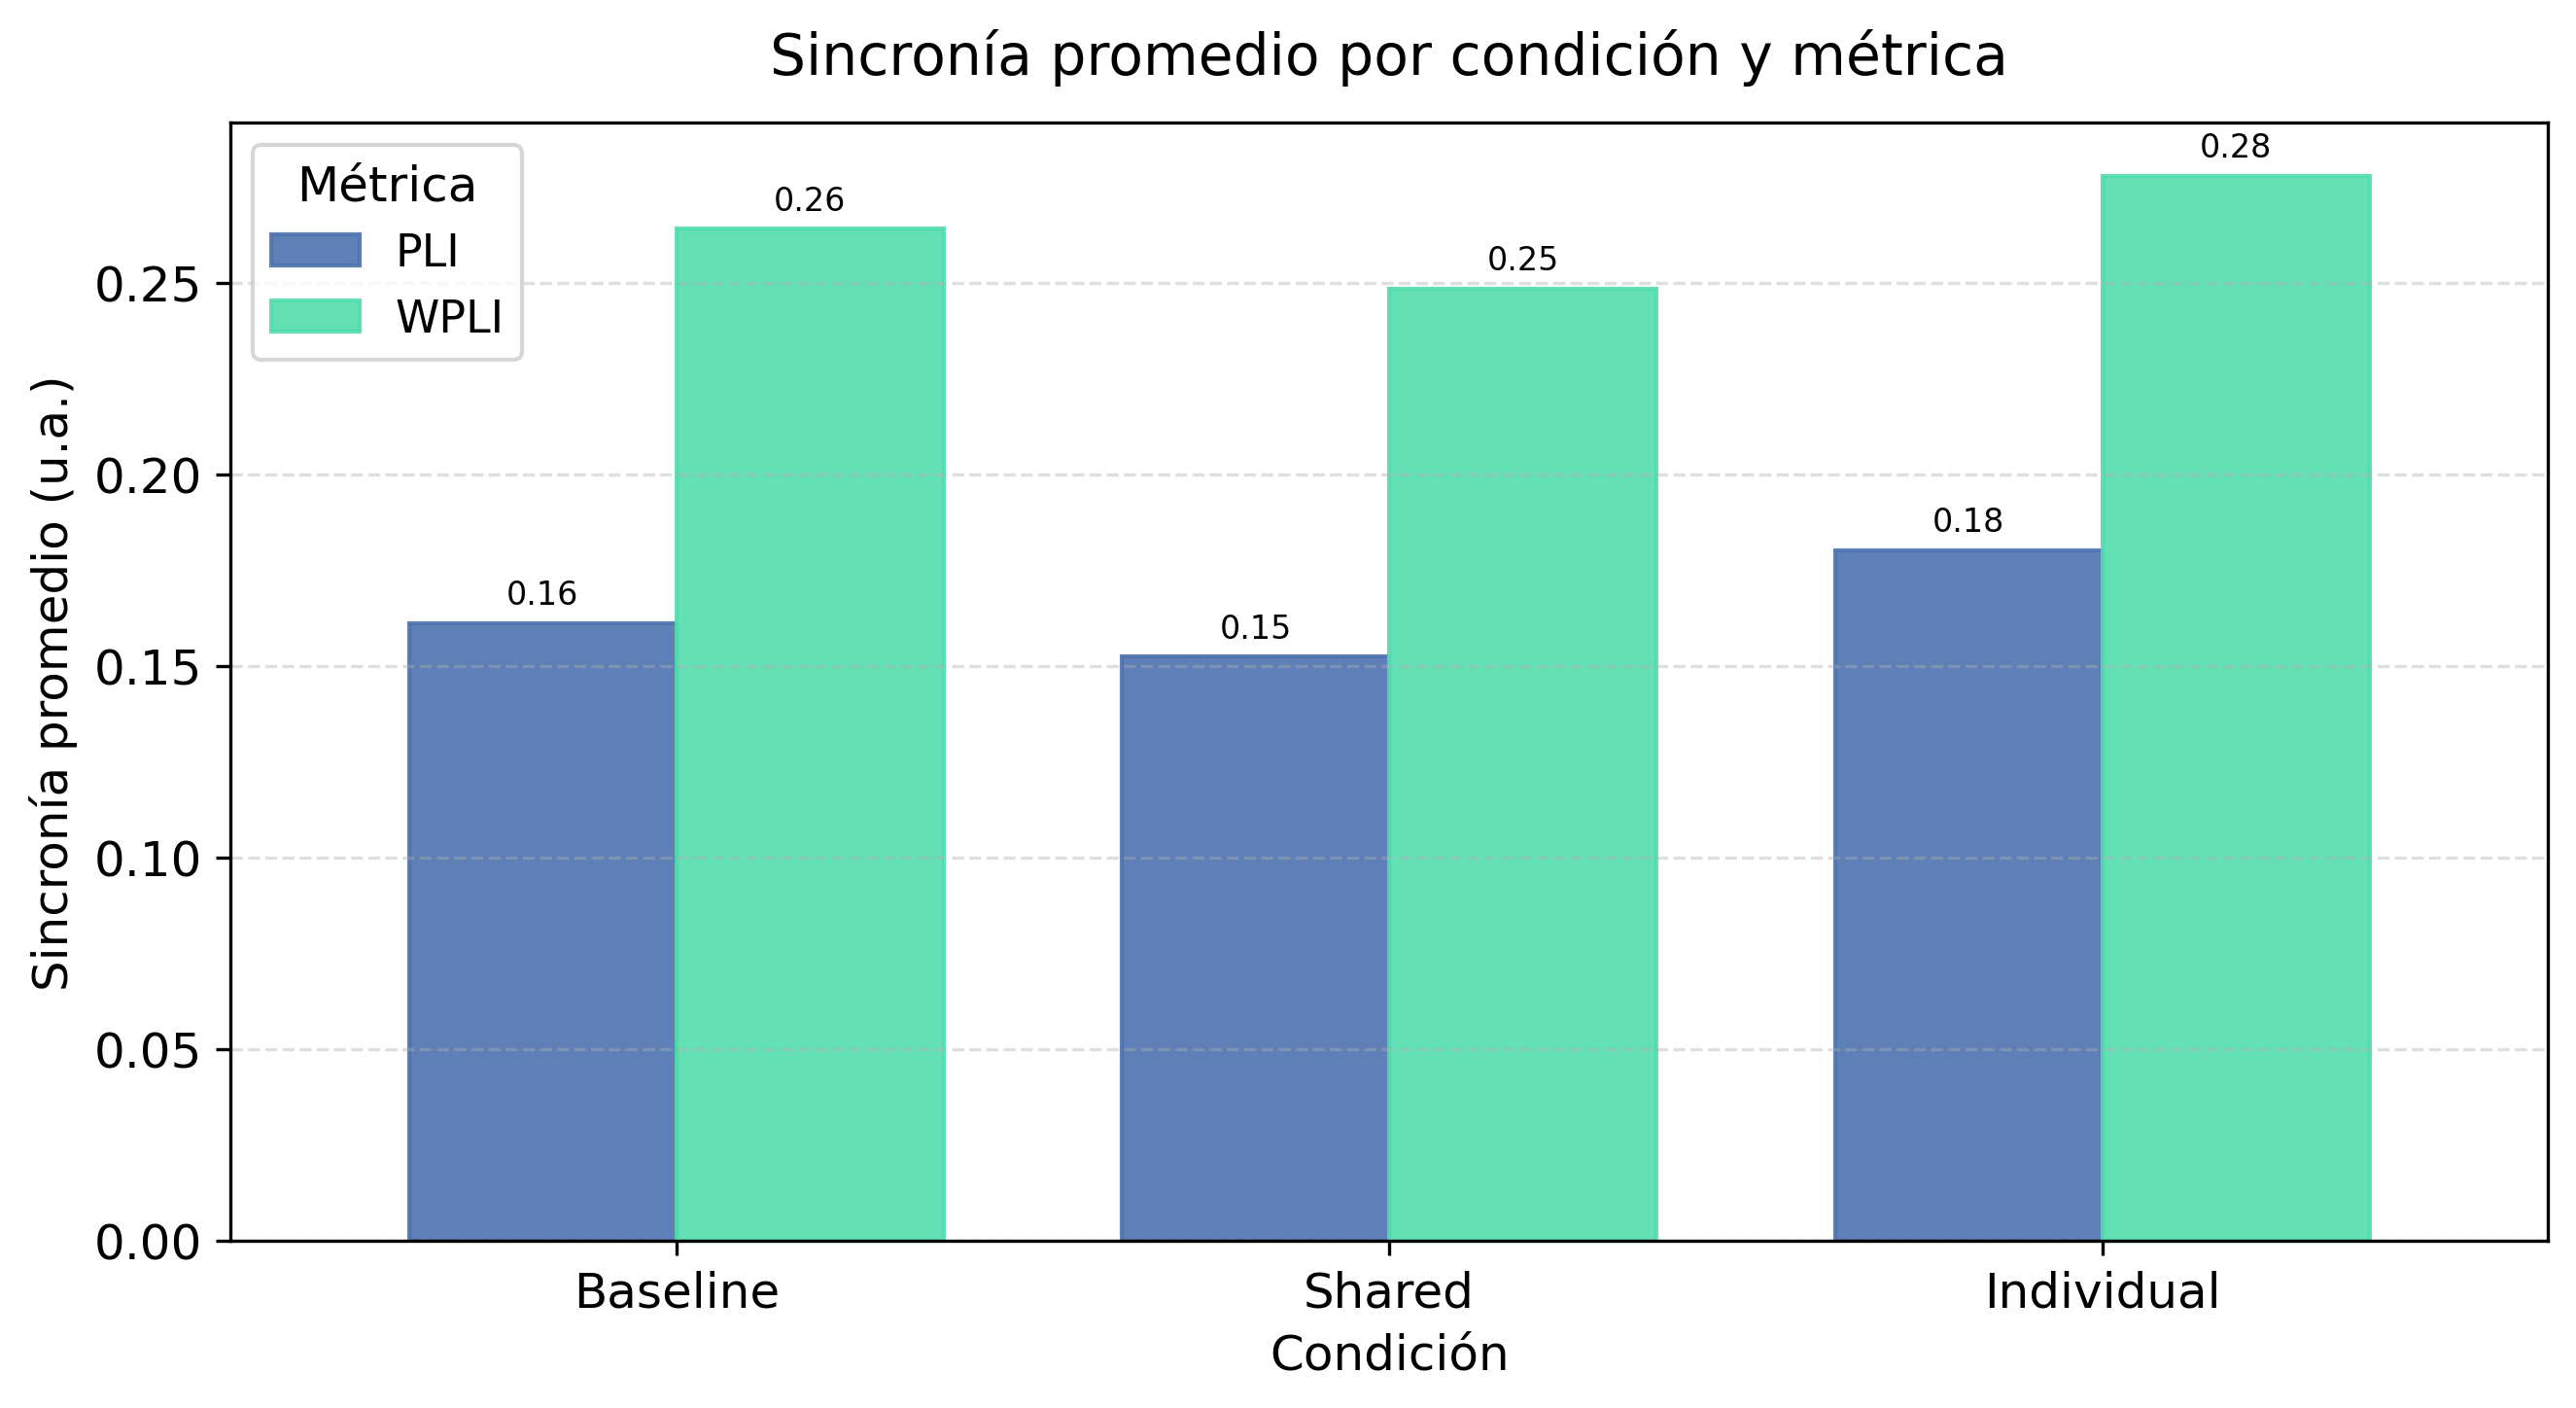
\includegraphics[width=0.8\textwidth]{figures/eda/condition_means.png}
    \caption{Sincronía promedio EEG por condición experimental (línea base, lectura compartida y lectura individual) y por métrica.}
\end{figure}

\begin{figure}[H]
    \centering
    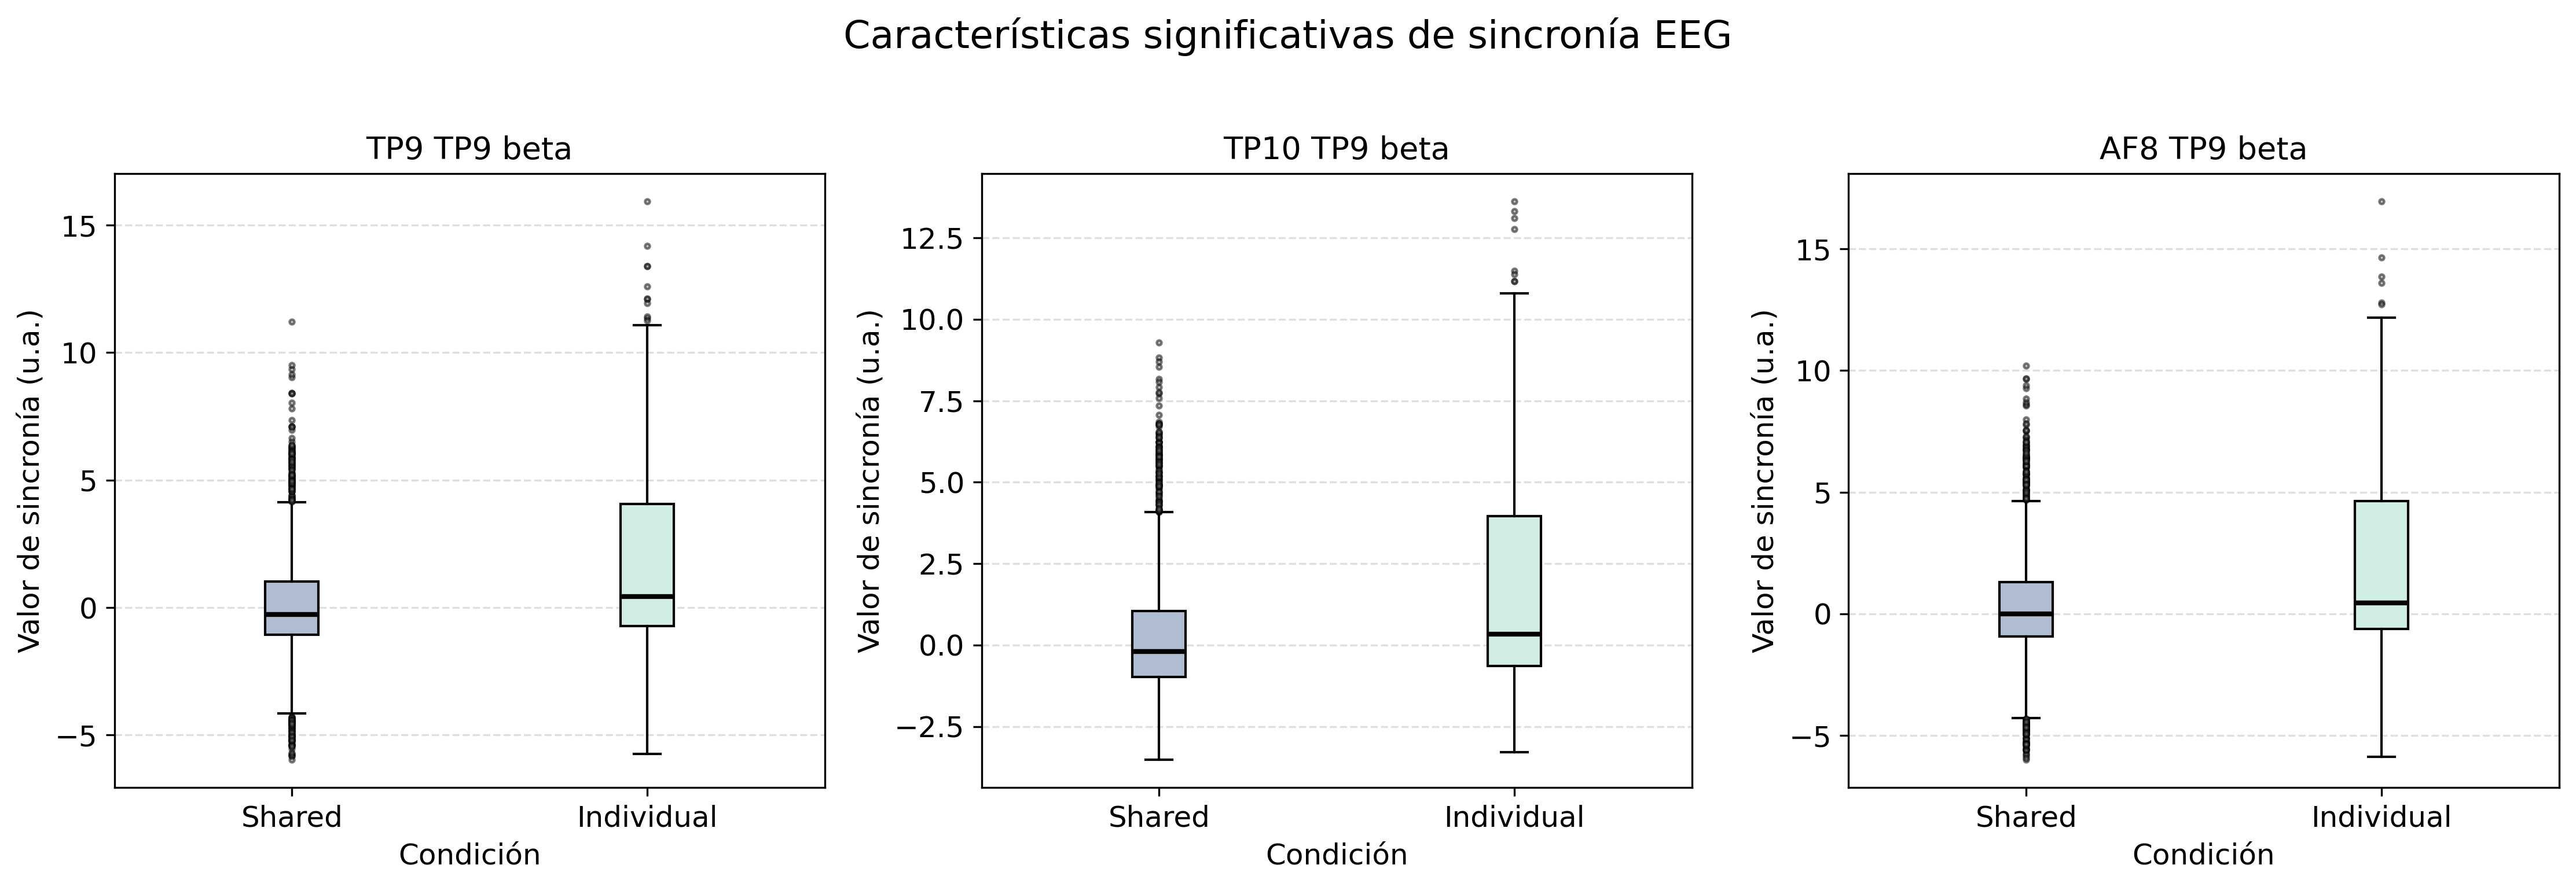
\includegraphics[width=0.95\textwidth]{figures/eda/boxplot_significant_features.png}
    \caption{Diagramas de caja de las características de sincronía EEG más significativas, comparando lectura compartida e individual.}
\end{figure}

\begin{figure}[H]
    \centering
    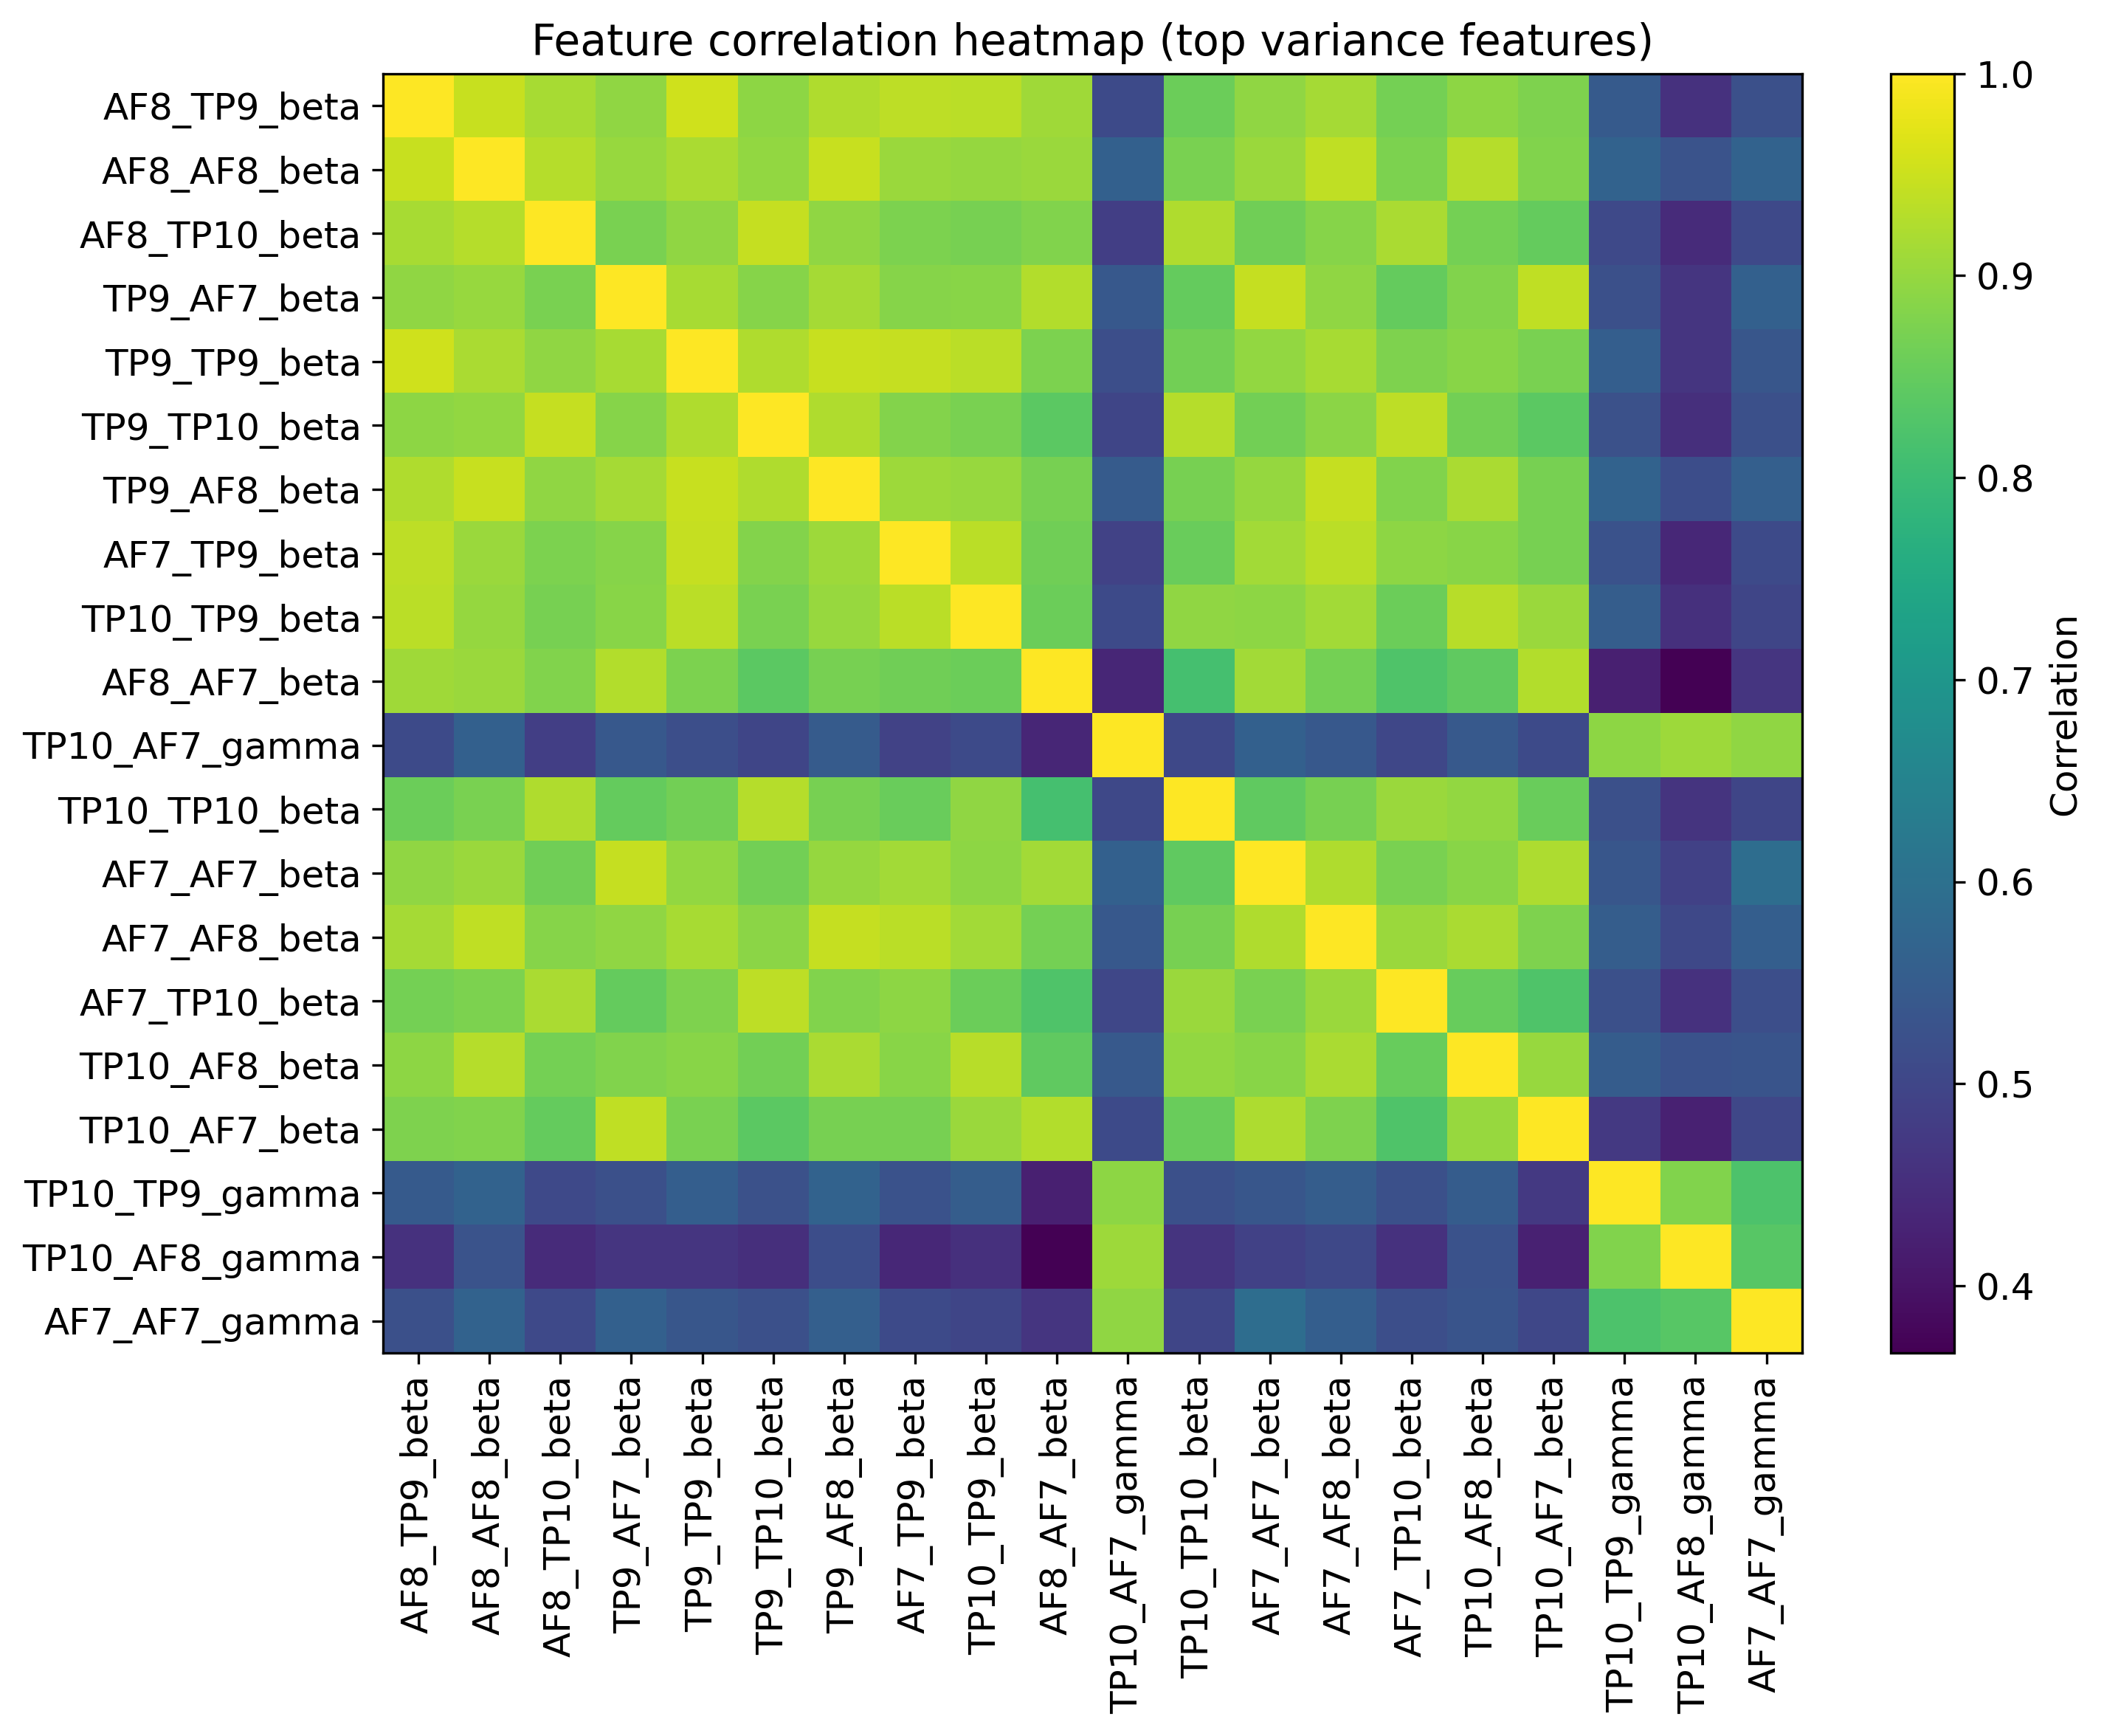
\includegraphics[width=0.9\textwidth]{figures/eda/feature_correlation_heatmap.png}
    \caption{Mapa de correlación de las características EEG con mayor varianza.}
\end{figure}

\section{Resultados de aprendizaje automático (C4)}
\begin{figure}[H]
    \centering
    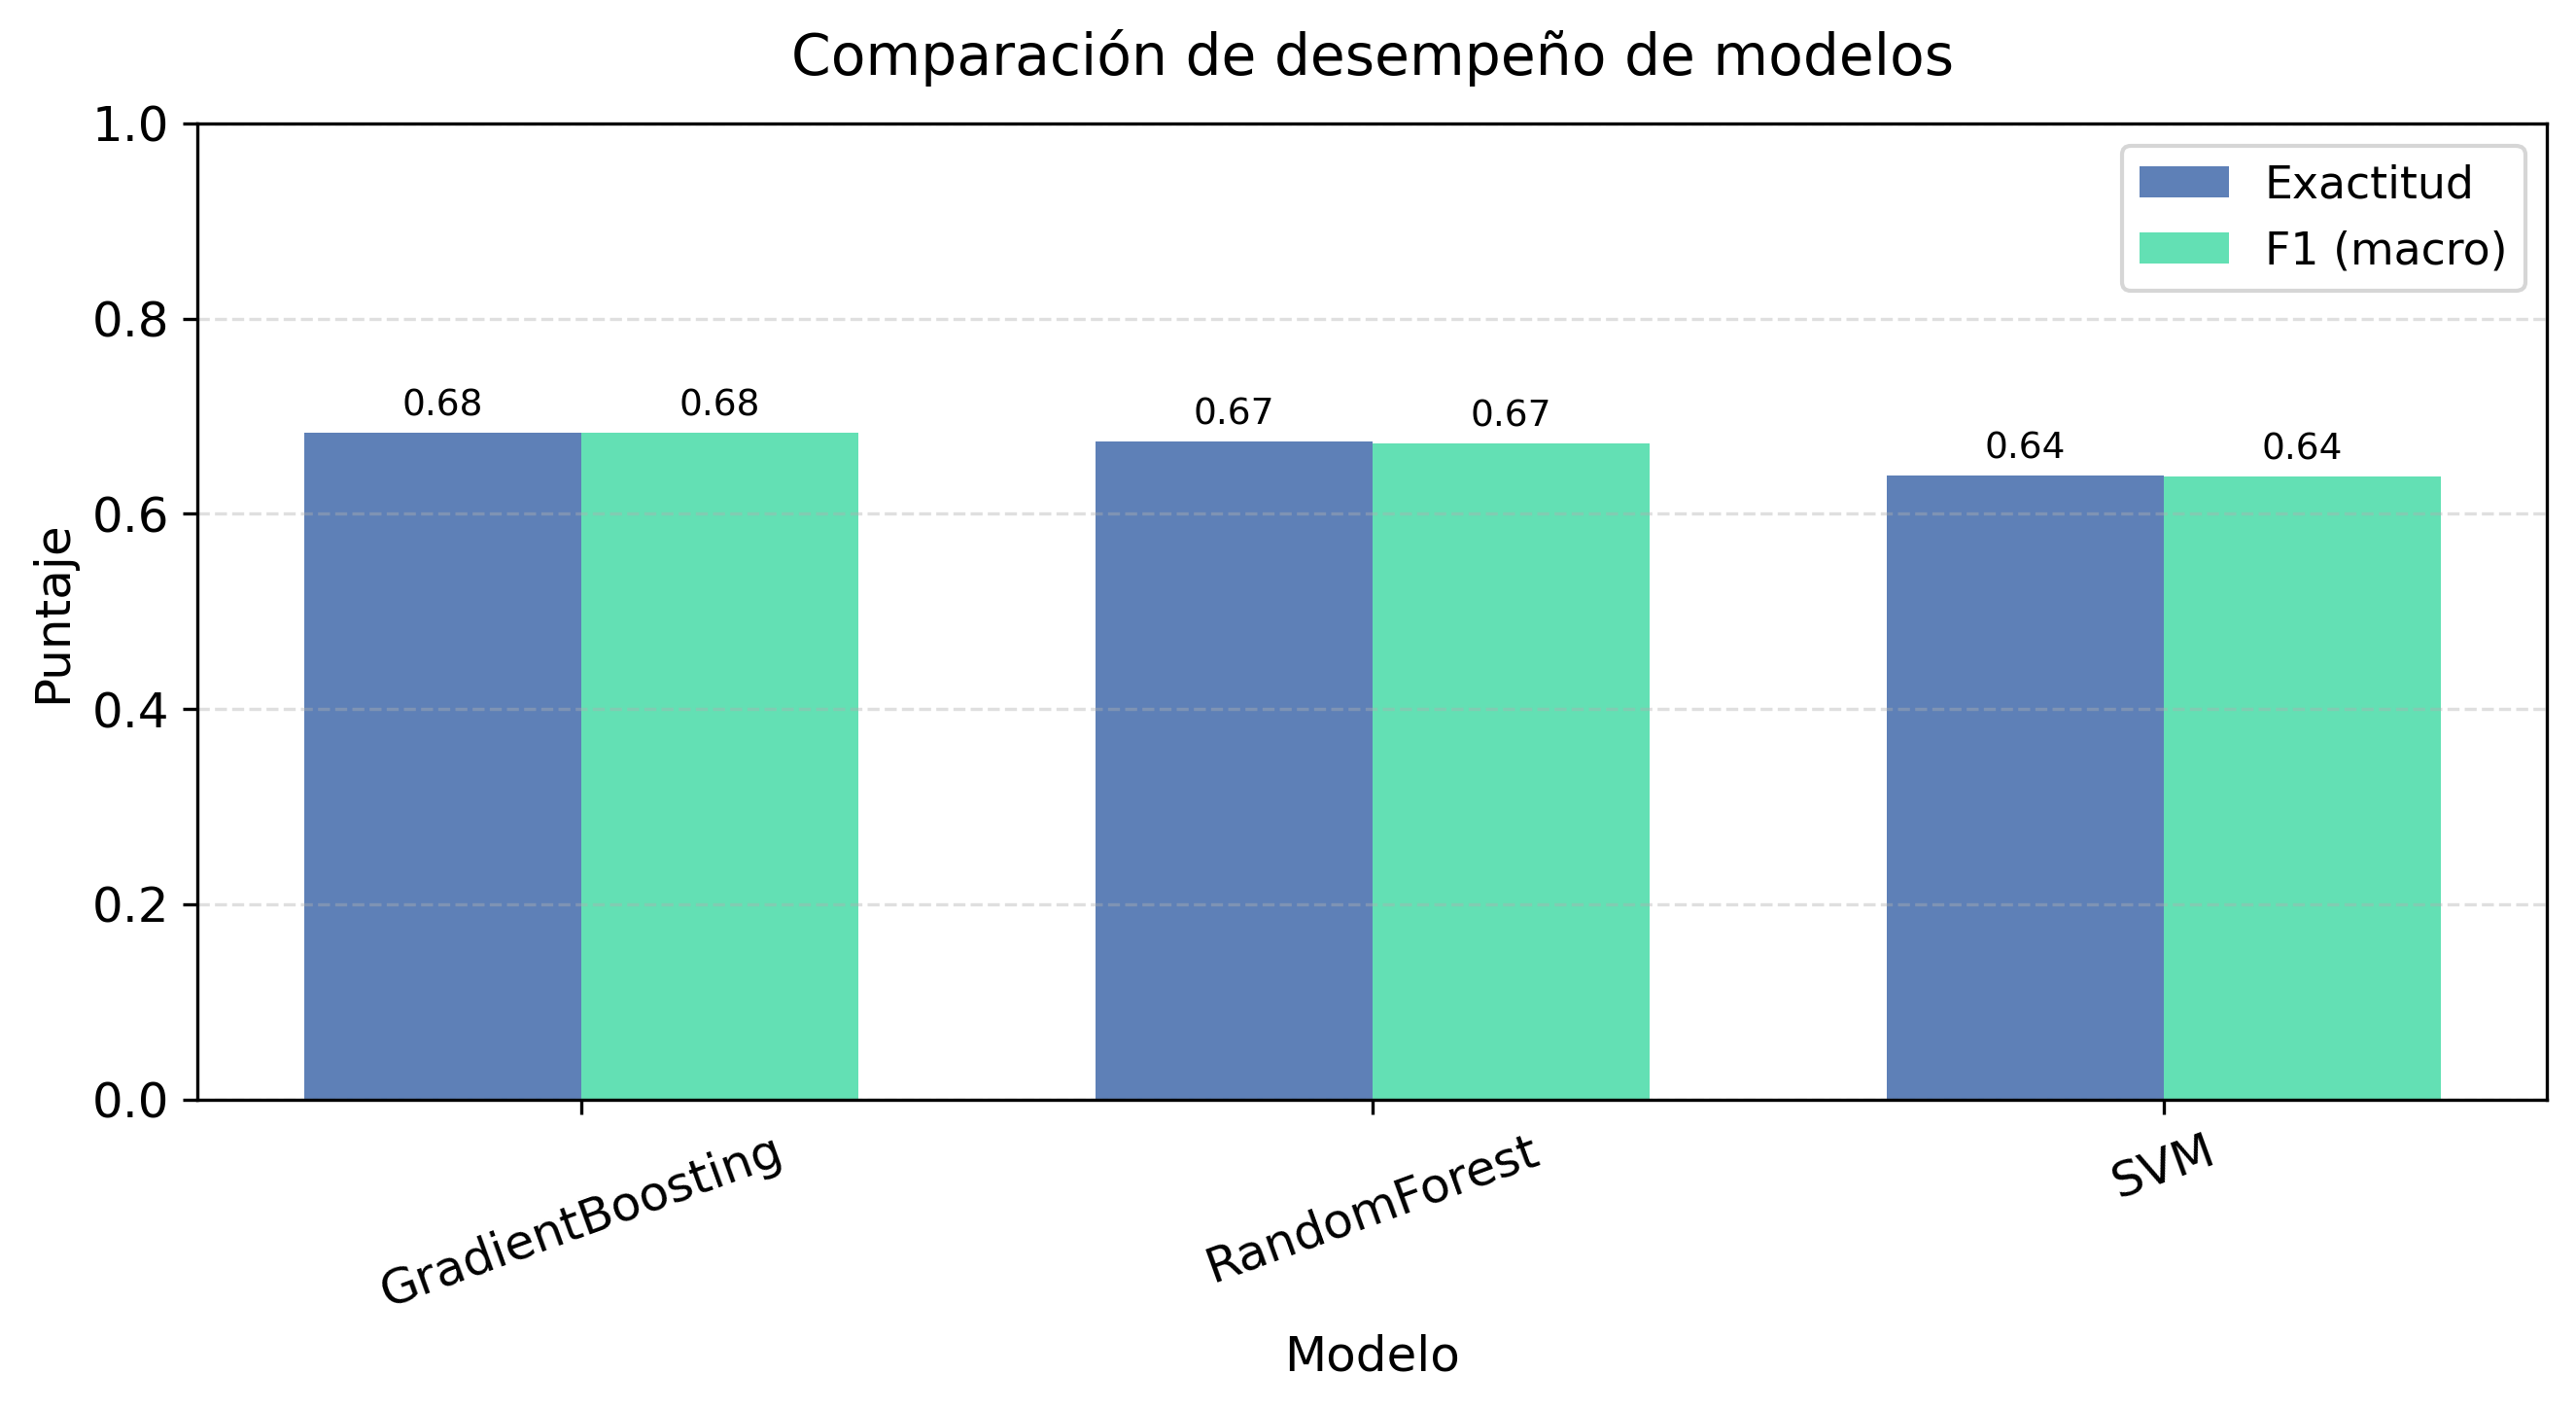
\includegraphics[width=0.8\textwidth]{figures/models/model_comparison.png}
    \caption{Comparación del desempeño de los modelos utilizando exactitud y F1 macro.}
\end{figure}

\begin{figure}[H]
    \centering
    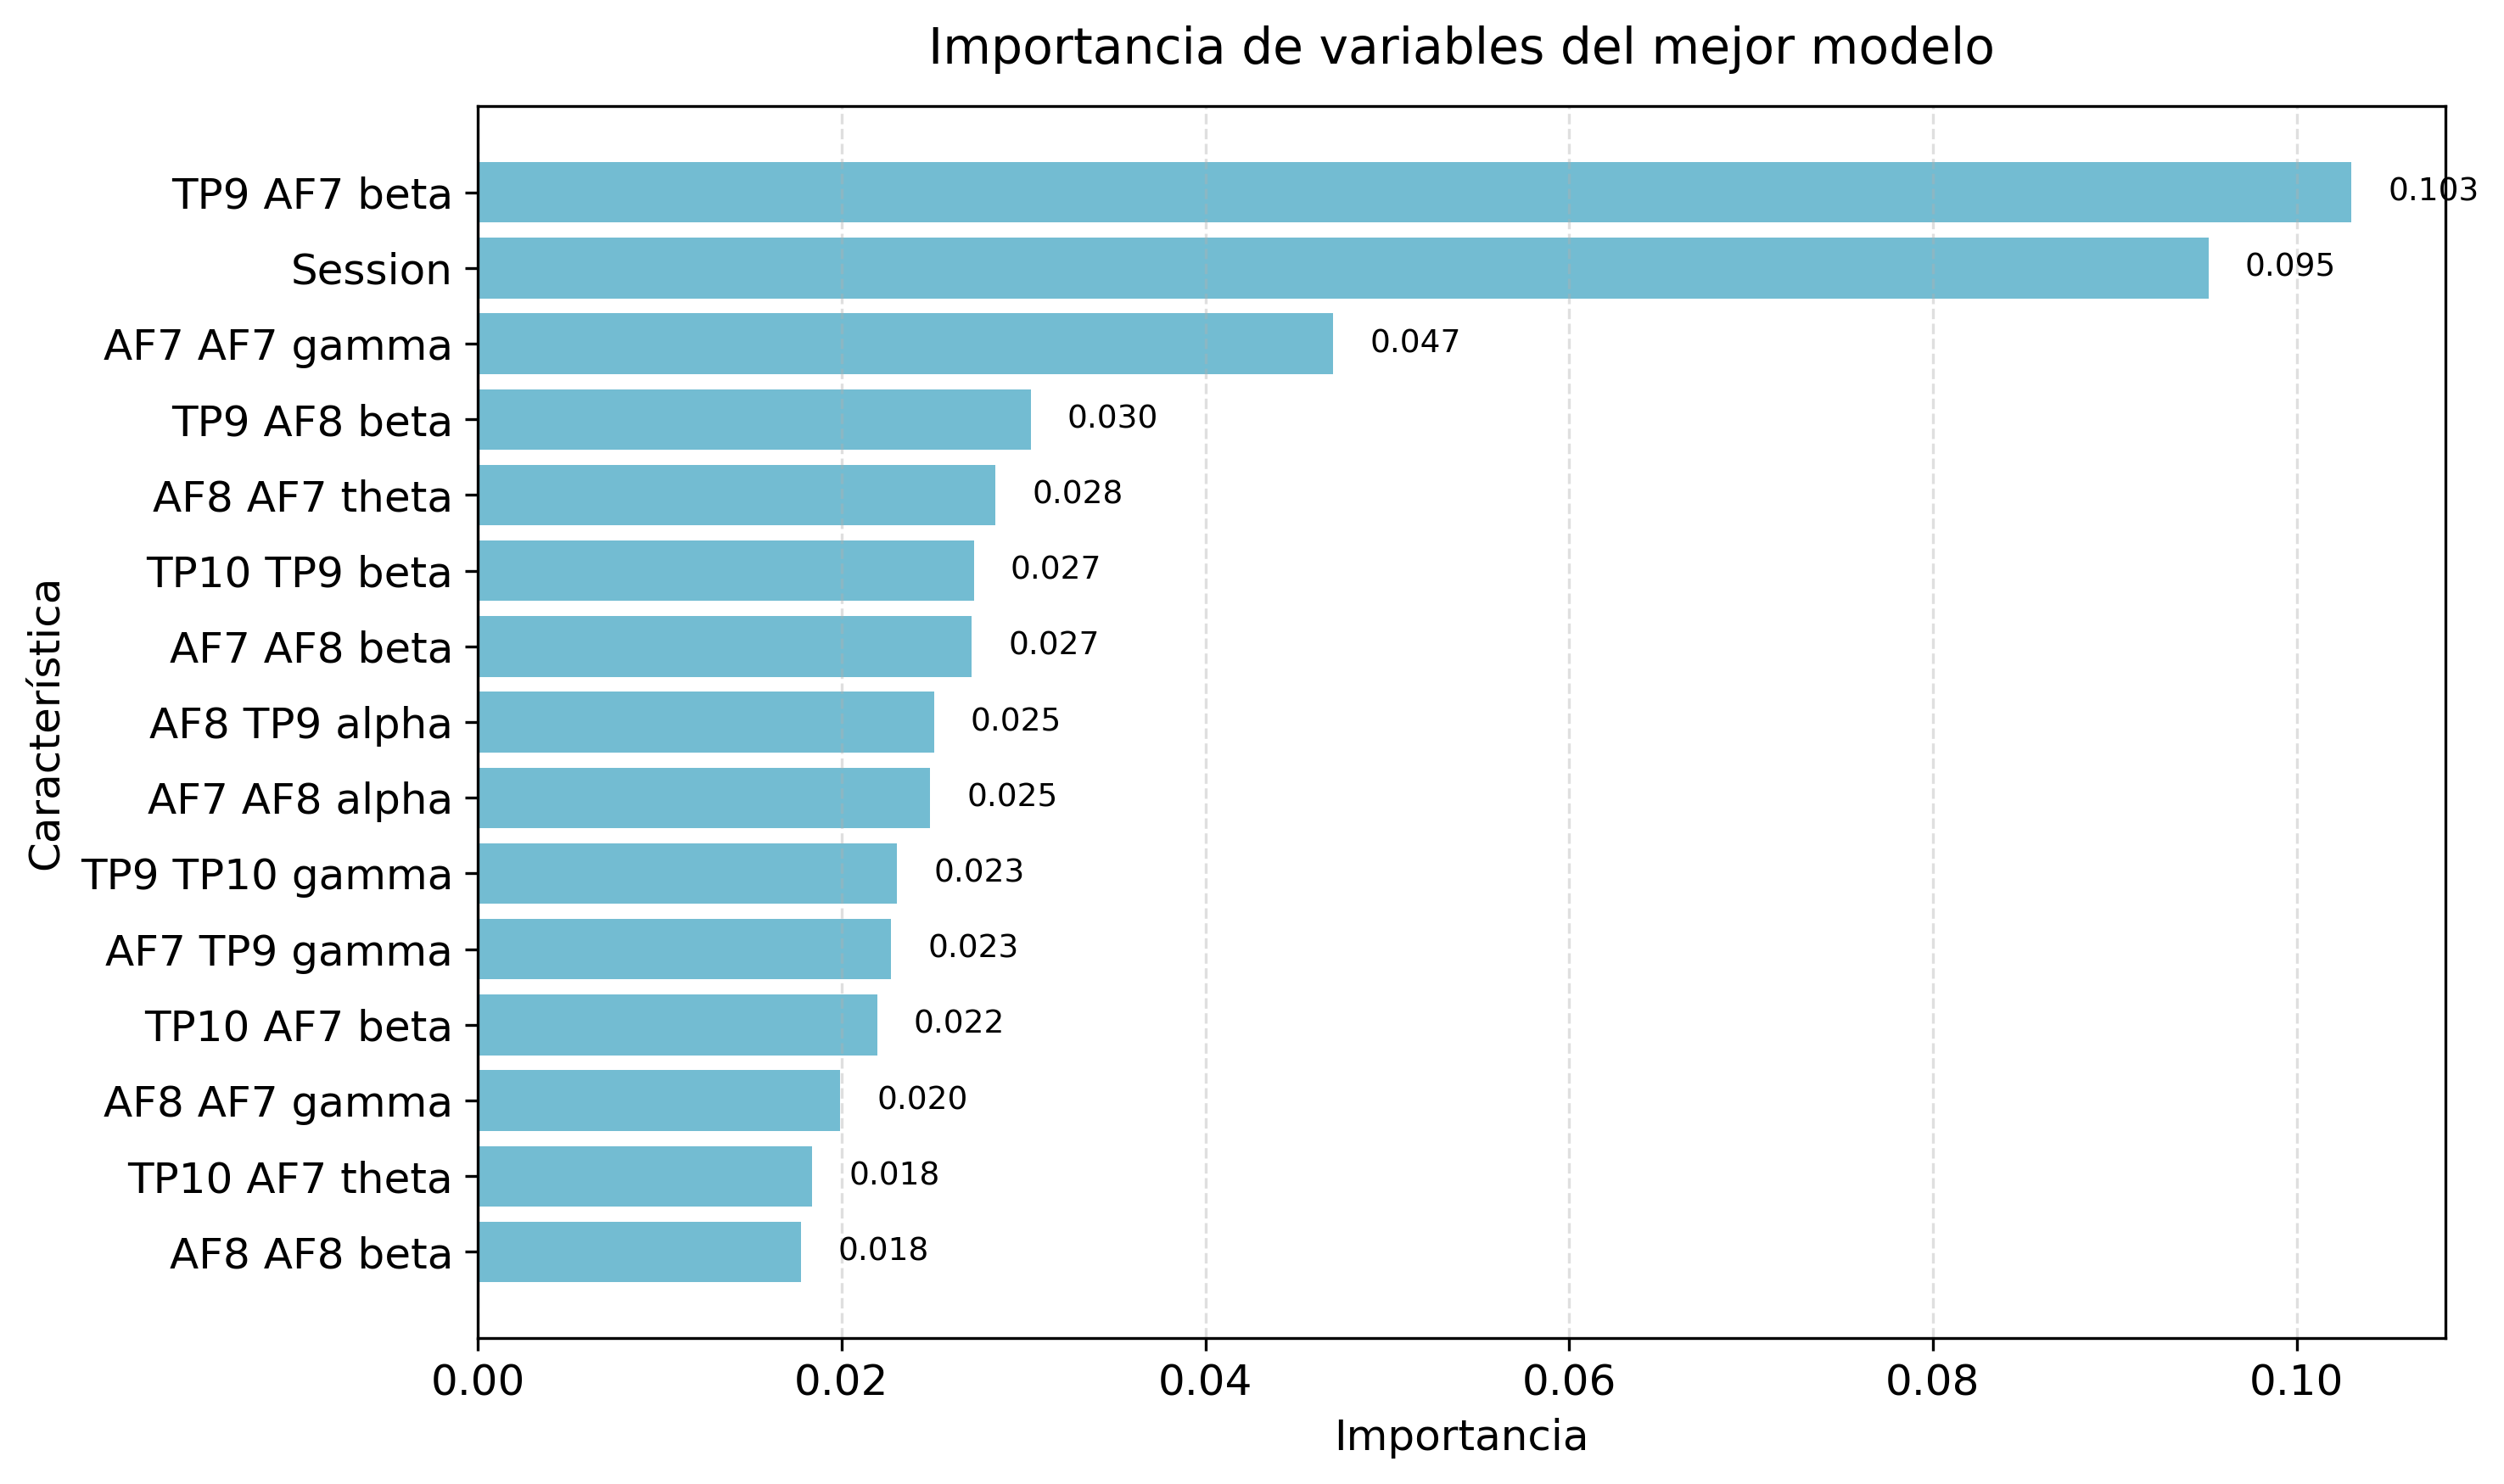
\includegraphics[width=0.9\textwidth]{figures/models/feature_importance.png}
    \caption{Importancia de variables en el modelo de mejor desempeño.}
\end{figure}

\section{Resultados de optimización (C3)}

\section{Tabla comparativa de modelos}
\begin{table}[H]
\centering
\caption{Comparación de desempeño entre modelos de aprendizaje automático.}
\begin{tabular}{lrrrr}
\toprule
Modelo & Exactitud & Precisión & F1 (macro) & F1 (ponderado) \\
\midrule
GradientBoosting & 0.683 & 0.683 & 0.683 & 0.683 \\
RandomForest & 0.674 & 0.674 & 0.672 & 0.673 \\
SVM & 0.639 & 0.638 & 0.638 & 0.638 \\
\bottomrule
\end{tabular}

\end{table}

\section{Conclusiones}

Texto

\end{document}
